%%
%
% ARQUIVO: anexo.tex
%
% VERSÃO: 1.0
% DATA: Maio de 2016
% AUTOR: Coordenação de Trabalhos Especiais SE/8
% 
%  Arquivo tex de exemplo de anexo do documento de Projeto de Fim de Curso.
%  Este exemplo traz dois anexos (dois comandos \chapter{•}). Poderiam ser colocados em arquivos .tex
%  separados. Neste caso, o arquivo main.tex deveria ter um \include{•} para cada arquivo .tex
%
% ---
% DETALHES
%  a. todo anexo deve começar com \chapter{•}
%  b. usar comando \noindent logo após \chapter{•}
%  c. segue os mesmos DETALHES do arquivo .tex de exemplo de capítulo do documento de Projeto de Fim de Curso
% ---
%%
\chapter{Descrição não formal da linguagem}
\noindent

LINGUAGEM HEADACHE (v 0.51b):\\
Formato livre \\
\textbf{Variáveis:} \\
tipos: byte, short e int. \\
\textbf{Constantes:}\\
tipos: byte e string.\\
\textbf{Funções:} 
\begin{verbatim}
    ret-type fuctionName(type parameter,…)
    void functionName(type parameter,…)
\end{verbatim} \\
\textbf{Operações:}

+,-,*,/,++,--  (byte,byte)

+,-,*,/,++,--  (short,short)

+,-,*,/,++,--  (int,int)

Nota: ++ e -- são comandos e não expressões.

Operações com inteiros que resultem em overflow são continuadas partindo do valor mínimo ou máximo.  \\
\textbf{Print}
\begin{verbatim}
    @ “string" 
    @int    //imprime inteiro 
    @byte   //imprime caractere ascii   
\end{verbatim}\\
autocast para int em caso de short.\\
\textbf{Input}
\begin{verbatim}
    #variável: lê da entrada padrão e adapta os bytes lidos ao tipo da variável 
    #byte //como caractere 
    #string //como string 
    #int //como inteiro 
\end{verbatim}\\
\textbf{Comandos:}
\begin{verbatim}
    if(condição) { 
        //Código 
    } 
    if (condição) { 
        //Código 
    } 
    else { 
        //Código 
    } 
    while(condição) { 
        //Código 
    } 
    for(begin;condição;end){ 
        //Código 
    } 
\end{verbatim}
\textbf{Condições:}
\begin{verbatim}
    int == int 
    int > int 
    int < int 
    int >= int 
    int <= int 
    int != int 
    cond && cond 
    cond || cond 
    (auto cast) 
\end{verbatim}
\textbf{Calls:}
\begin{verbatim}
   functionName(Arguments);  
\end{verbatim}\\
\textbf{Modelo de memória:} 

Funções estáticas inline.  

Não há recursão.

Cada definição de função reserva a área da função. 

A área da função é composta de suas variáveis, mais a área necessária para os temporários de suas expressões.

Parâmetros são transformados em variáveis ordinárias. 

Não há ponteiros. 

Não há memória dinâmica.



\chapter{EBNF de Headache}
\noindent
program: {definition}\\
definition: def-var | def-func\\
def-var : type nameList ';'\\
nameList: ID { ',' ID }\\
type : baseType | type '[' ']'\\
baseType : byte | short | int \\
command:

\begin{verbatim}
    IF '(' exp ')' command [ ELSE command ]
    | WHILE '(' exp ')' command
    | FOR (command; exp; command)
    | var '=' exp ';'
    | RETURN [ exp ] ';'
    | call ';'
    | '@' exp ';'
    | var++;
    | var--;
    | '#' var ‘;’
    | ‘%' ‘;'
    | block

    var : ID | exp '[' exp ']'
    exp : NUMERAL | LITERAL
    | var
    | '(' exp ')'
    | call
    | exp 'as' tipo
    | '-' exp
    | exp '+' exp
    | exp '-' exp
    | exp '*' exp
    | exp '/' exp
    | exp '==' exp
    | exp '<=' exp
    | exp '>=' exp
    | exp '<' exp
    | exp '>' exp
    | '!' exp
    | exp '&&' exp
    | exp '||' exp
    call: ID '(' expList ')'
    expList : [ exp { ',' exp } ]
\end{verbatim}

\chapter{Descrição breve de brainfuck}

Brainfuck é uma linguagem de programação Turing Complete composta por apenas 8 caracteres. São eles: ‘>’, ‘<’ , ‘+’, ‘-’, ‘,’ , ‘.’ , ‘[’, ‘]’ 
Cada um deles representa um comando específico. São eles:

>\hspace*{1.5cm}ir a direita

<\hspace*{1.5cm}ir a esquerda

+\hspace*{1.5cm}incrementar corrente

-\hspace*{1.5cm}decrementar corrente 

,\hspace*{1.5cm}input na célula corrente

.\hspace*{1.5cm}output na célula corrente

[\hspace*{1.5cm}abre while loop

]\hspace*{1.5cm}fecha while loop


Um programa Brainfuck roda numa memória compostas de células de 8 bits. A especificação mais comum é uma memória de 30000 células de 8 bits. Quando um programa começa a memória deve estar com todas as suas células zeradas, e a célula corrente deve ser a célula de número zero. A especificação também prevê que não haja nenhuma célula à esquerda da célula zero: Uma instrução ‘<’ quando o programa está na célula zero de memória deve gerar um erro em um interpretador de brainfuck.
Um programa brainfuck com loops  ('[ ' e ']') desbalanceados são undefined behavior em brainfuck. No artefato bfi implementado, a decisão foi gerar um erro.
Formalmente, brainfuck é definida com a seguinte tradução para C:

\begin{figure}[h]
    \centering
	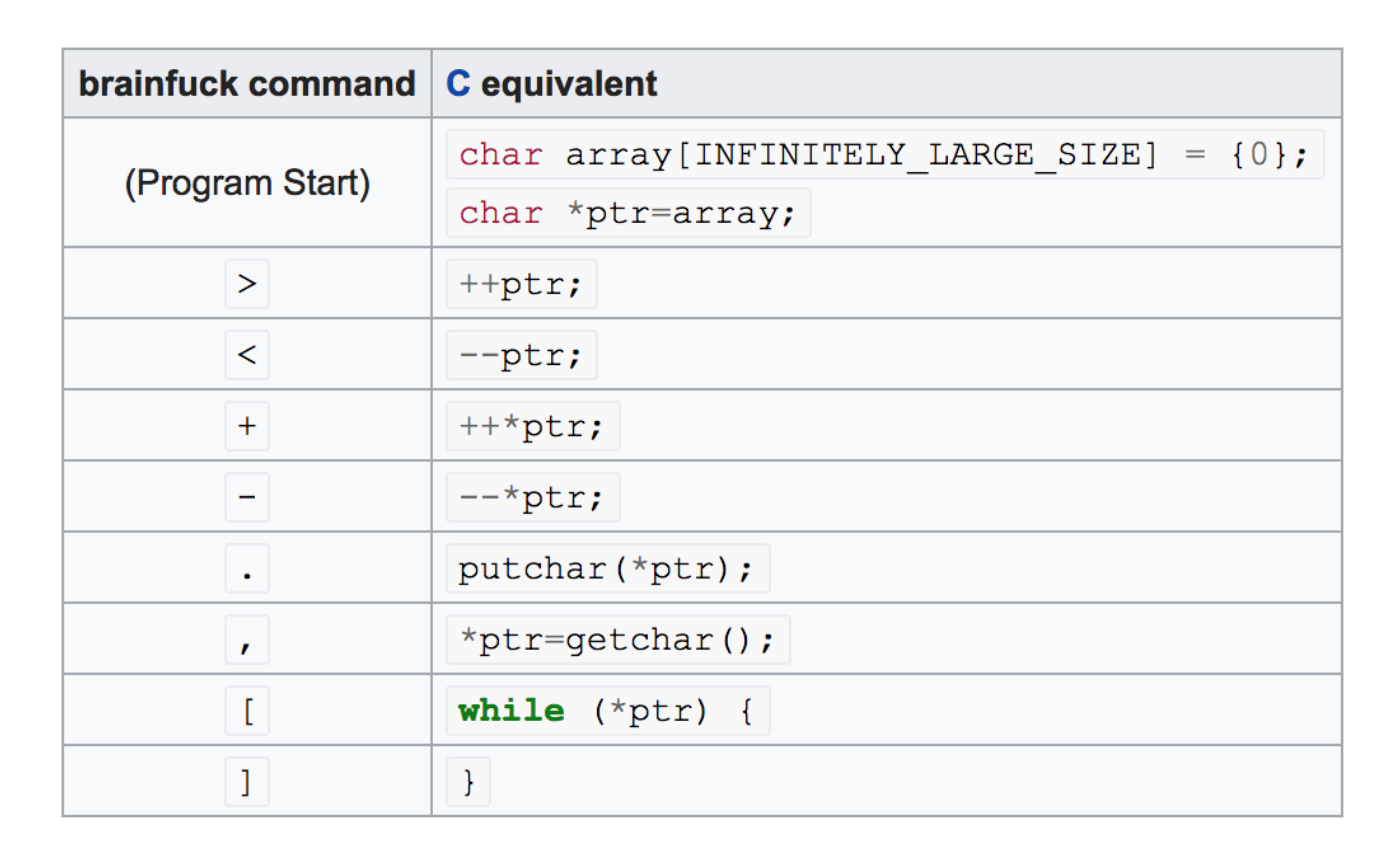
\includegraphics[width = 10cm]{TD/img/C.png}
	\caption{Tradução do brainfuck para o C}
	\label{traducao}
\end{figure}

\chapter{Instruções de Uso}

Essa instrução é dedicada àqueles que executarão o código no CD

\begin{itemize}
    \item Ler o README.txt
    \item Para rodar o "make testrunnable" no linux é necessário executar "git checkout linux" 
    \item Consultar a wiki de Headache em caso de dúvida (https://github.com/LucasMW/Headache/wiki)
    \item Digitar "git pull" para atualizar o projeto
\end{itemize}